% F3: running-intersection schematic and the actual cycle's conflicting cell.
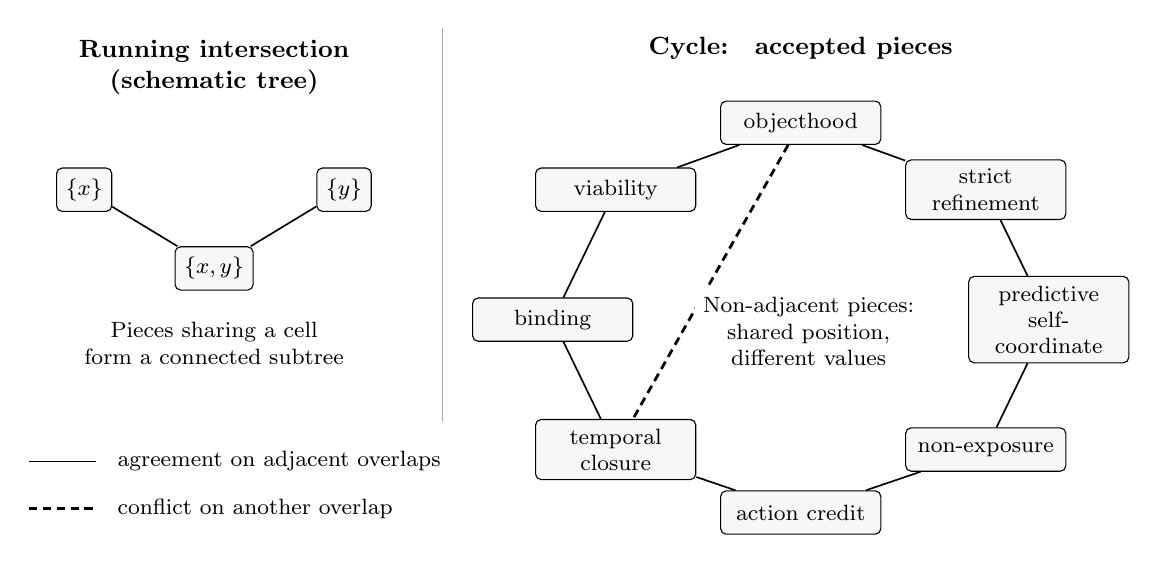
\begin{tikzpicture}[x=1cm,y=1cm,font=\footnotesize,
 piece/.style={draw,rounded corners=2pt,fill=black!3,align=center,minimum height=.55cm},
 adjacent/.style={semithick},conflict/.style={densely dashed,line width=1pt}]
\node[font=\small\bfseries,align=center] at (2.65,3.45) {Running intersection\\(schematic tree)};
\node[piece] (a) at (1,1.9) {$\{x\}$};
\node[piece] (b) at (2.65,.9) {$\{x,y\}$};
\node[piece] (c) at (4.3,1.9) {$\{y\}$};
\draw[adjacent] (a)--(b)--(c);
\node[align=center] at (2.65,-.05) {Pieces sharing a cell\\form a connected subtree};
\draw[black!35] (5.55,-1.05)--(5.55,3.95);
\node[font=\small\bfseries] at (10.1,3.7) {Cycle: \snapPosZeroFourStagedClauseCount{} accepted pieces};
\node[piece,text width=1.8cm] (obj) at (10.1,2.75) {objecthood};
\node[piece,text width=1.8cm] (refine) at (12.45,1.9) {strict\\refinement};
\node[piece,text width=1.8cm] (predict) at (13.25,.25) {predictive\\self-coordinate};
\node[piece,text width=1.8cm] (privacy) at (12.45,-1.4) {non-exposure};
\node[piece,text width=1.8cm] (credit) at (10.1,-2.2) {action credit};
\node[piece,text width=1.8cm] (time) at (7.75,-1.4) {temporal closure};
\node[piece,text width=1.8cm] (binding) at (6.95,.25) {binding};
\node[piece,text width=1.8cm] (viable) at (7.75,1.9) {viability};
\draw[adjacent] (obj)--(refine)--(predict)--(privacy)--(credit)--(time)--(binding)--(viable)--(obj);
\draw[conflict] (obj)--(time);
\node[align=center,fill=white,inner sep=3pt] at (10.2,.1) {Non-adjacent pieces:\\shared position,\\different values};
\draw[adjacent] (.3,-1.55)--(1.15,-1.55);
\node[anchor=west] at (1.3,-1.55) {agreement on adjacent overlaps};
\draw[conflict] (.3,-2.15)--(1.15,-2.15);
\node[anchor=west] at (1.3,-2.15) {conflict on another overlap};
\end{tikzpicture}
